\section{Training Approach}

\begin{outline}
  Describe the reinforcement learning or supervised learning approach used to train the CNN models.
\end{outline}

\[
  \mathbf{s} = \begin{bmatrix}
    \mathbf{p} \\
    \mathbf{q_r} \\
    \mathbf{v} \\
    \mathbf{\omega} \\
  \end{bmatrix} \in \mathbb{R}^{12}
\]

\[
  \mathbf{x} = \begin{bmatrix}
    \mathbf{q} \\
    \mathbf{\dot q} \\
    \mathbf{s} \\
    \mathbf{u}
  \end{bmatrix}
\]

\begin{figure}
  \centering
  \begin{minipage}[T]{0.45\textwidth}
    \centering
    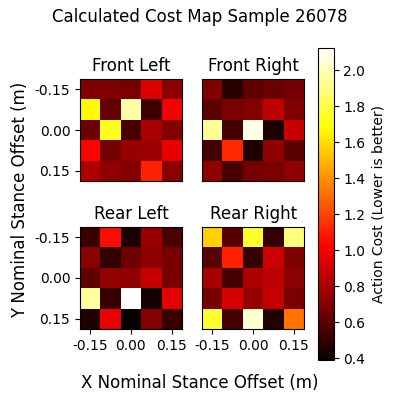
\includegraphics[width=\textwidth]{images/data/training/calculated-quadruped_2025-09-19T08-16-04.png}
  \end{minipage}
  \hfill
  \begin{minipage}[T]{0.45\textwidth}
    \centering
    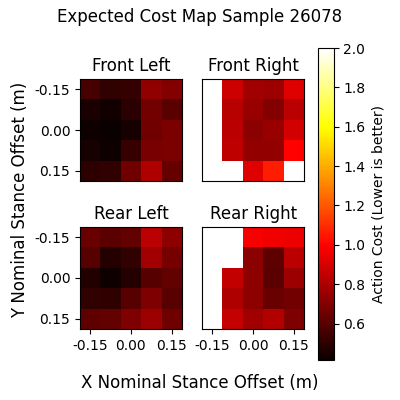
\includegraphics[width=\textwidth]{images/data/training/expected-quadruped_2025-09-19T08-16-04.png}
  \end{minipage}
  \hfill

  \caption{Training data samples showing calculated (left) and expected (right) quadruped images.}
  \label{fig:data-training-data-samples}
\end{figure}